\begin{frame}
  \frametitle{\problemtitle}

  \begin{columns}
    \begin{column}[T]{.70\textwidth}
      \begin{itemize}
      \item Given is a fraction $a/b$,
        try to make it equal to $c/d$ by
        cancelling some digits in $a$ and $b$
        ($1\leq a,b,c,d< 10^{18}$).
      \item If possible, print the leftover digits.
      \item If it is impossible, print ``\texttt{impossible}''.
      \end{itemize}
    \end{column}

    \illustration{0.3}{meme.png}{Source: The Internet\texttrademark.\vspace{-6em}}%
  \end{columns}

  \centering
  \vspace{3em}
  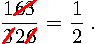
\includegraphics[trim={0 0 1ex 0},clip,width=0.15\textwidth]{fraction1-half.pdf}

  \small Illustration of Sample Input 1, where you can cancel digits $3$ and $6$ from $163/326$ to obtain $1/2$.
\end{frame}
